\clearpage
\section{Praktijkvoorbeeld: Grote Markt in Sint-Niklaas}
\label{sec:voorbeeld-grote-markt}

Voor deze praktijkproef werd handmatig een foto geselecteerd van een druk moment tijdens de feestelijke inhuldiging van de Grote Markt in Sint-Niklaas. Het beeld toont een grote groep bezoekers, met vooral centraal en rechts veel personen dicht bij elkaar. De oorspronkelijke foto heeft een hoge resolutie van \(5120 \times 3415\) pixels en een goede belichting. Daardoor zijn veel afzonderlijke hoofden herkenbaar, al bemoeilijken de onderlinge overlap en de boom in het midden van het beeld een volledige telling.

\subsection{Handmatige telling}

Als referentie werd eerst een handmatige telling uitgevoerd op de oorspronkelijke foto. Daarbij werden 738 hoofden aangeduid. Deze telling wordt als een onderschatting beschouwd. Twijfelgevallen zijn niet overal volledig of eenduidig gemarkeerd, bijvoorbeeld wanneer dicht opeengepakte hoofden alleen door een verschil in haarkleur van elkaar te onderscheiden zijn. Ook personen die gedeeltelijk achter de boom staan, zijn niet allemaal aangeduid. Het werkelijke aantal aanwezigen ligt naar inschatting van de auteur daarom hoger dan de ongeveer 738 getelde personen.

\begin{figure}[htbp]
    \centering
    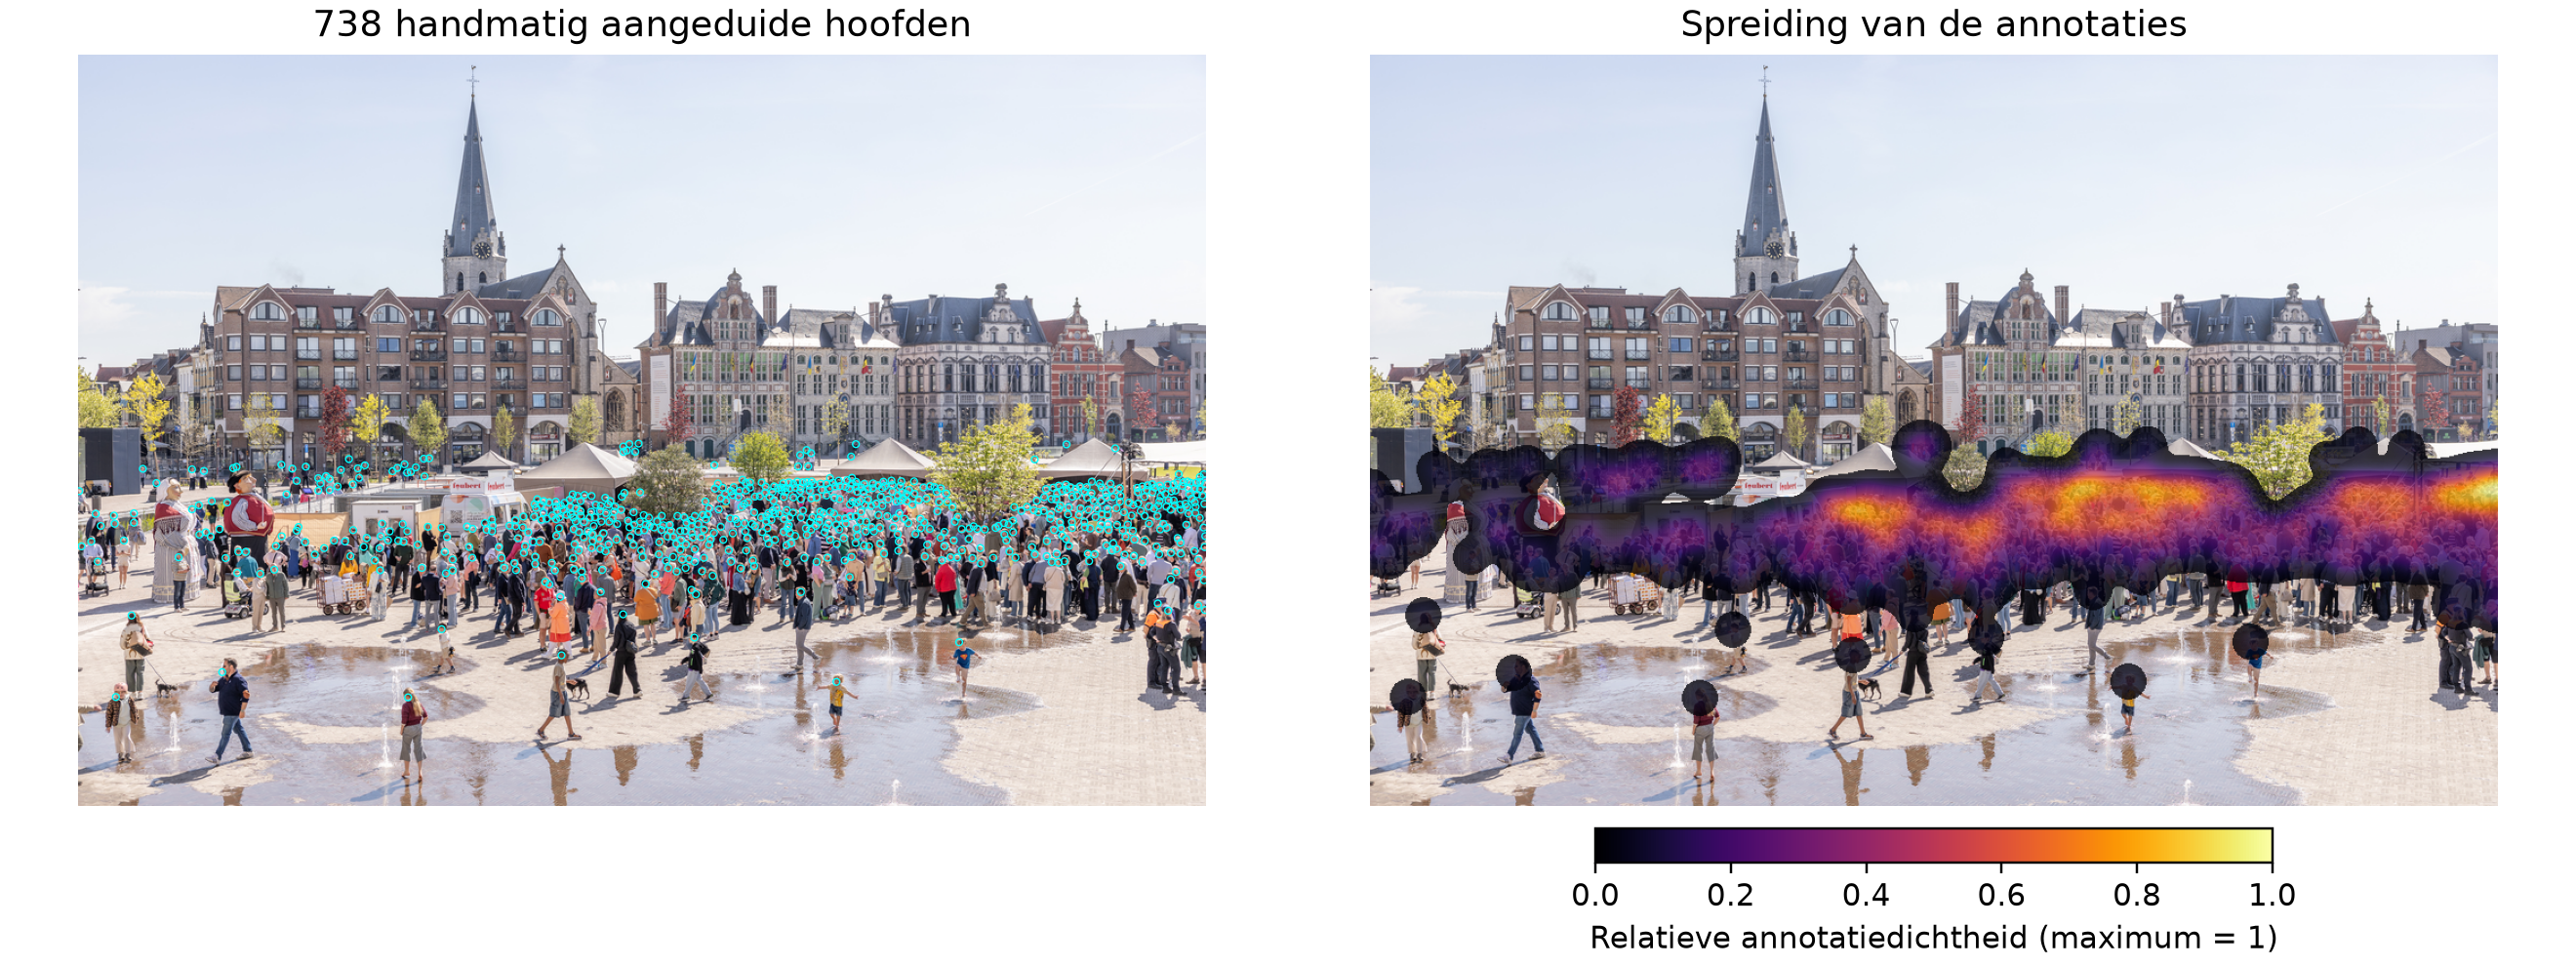
\includegraphics[width=\textwidth]{voorbeelden/grote-markt-sint-niklaas/handmatige-telling.png}
    \caption[Grote Markt: handmatige telling en annotatieheatmap]{De geselecteerde evenementfoto met links de 738 handmatig aangeduide hoofden en rechts de bijbehorende heatmap. Warme kleuren duiden op een hogere concentratie van annotaties. Zones zonder markeringen zijn niet noodzakelijk leeg. Foto: Stad Sint-Niklaas \autocite{SintNiklaas2026GroteMarkt}; annotaties: eigen telling.}
    \label{fig:grote-markt-handmatig}
\end{figure}

De export van de telling bevat de coördinaten van alle 738 markeringen. Voor de heatmap in Figuur~\ref{fig:grote-markt-handmatig} zijn deze punten naar een raster van \(1024 \times 683\) pixels geschaald en afgevlakt met een Gaussische kernel met \(\sigma=10\) pixels. De numerieke map behoudt een som van 738; voor de kleurweergave is het maximum op 1 gezet. De heatmap toont de spreiding van de aangeduide hoofden in het beeld en geeft geen fysieke dichtheid in personen per vierkante meter.

\clearpage
\subsection{Modelvoorspelling en vergelijking}

Van de vier onderzochte CSRNet-varianten komt het model uit de finale trainingsrun het dichtst bij de handmatige telling. Zelfs dit model voorspelt slechts ongeveer 544 personen. Dat is ongeveer 194 personen of \(26{,}3\%\) minder dan de 738 aangeduide hoofden. De beste modelvoorspelling ligt dus aanzienlijk onder een telling die zelf al een onderschatting is. Het checkpoint uit epoch 39 werd geselecteerd op basis van de laagste validatiefout op ShanghaiTech Part B.

Voor de daadwerkelijke inferentie werd de foto proportioneel verkleind van \(5120 \times 3415\) tot \(1024 \times 683\) pixels, zonder uitsnede. Hierdoor gaat detail verloren, vooral bij kleine hoofden en dicht opeengepakte groepen. Dit kan bijdragen aan de onderschatting, maar het effect van de invoerresolutie is niet afzonderlijk gemeten.

\begin{figure}[htbp]
    \centering
    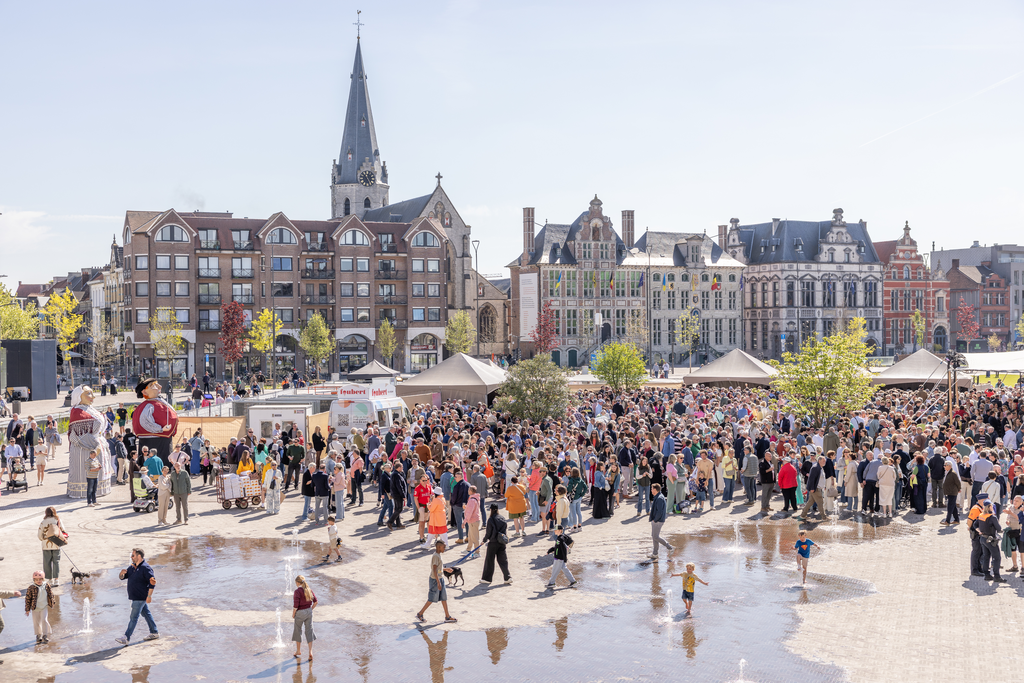
\includegraphics[width=0.49\textwidth]{voorbeelden/grote-markt-sint-niklaas/invoer.png}\hfill
    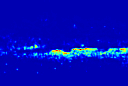
\includegraphics[width=0.49\textwidth]{voorbeelden/grote-markt-sint-niklaas/beste-heatmap.png}
    \caption[Grote Markt: modelinvoer en voorspelde density map]{Links: de verkleinde foto die als modelinvoer dient. Rechts: de density map van het geselecteerde CSRNet-model, met een voorspelling van ongeveer 544 personen. De kleuren zijn relatief aan deze map en kunnen niet rechtstreeks worden vergeleken met die van de handmatige heatmap. Foto: Stad Sint-Niklaas \autocite{SintNiklaas2026GroteMarkt}.}
    \label{fig:grote-markt-voorspelling}
\end{figure}

\begin{table}[htbp]
    \centering
    \small
    \begin{tabular}{lrrr}
        \toprule
        \textbf{CSRNet-variant} & \textbf{Epoch} & \textbf{Personen} & \textbf{Tijd (ms)} \\
        \midrule
        % Generated by crowd_counting/example_grote_markt.py
CPU-kalibratie & 1 & \(295{,}7\) & \(96{,}43\) \\
GPU-kalibratie & 1 & \(353{,}0\) & \(96{,}66\) \\
Gecontroleerde run, 1 epoch & 1 & \(255{,}8\) & \(96{,}93\) \\
Finale run, 100 epochs & 39 & \(544{,}2\) & \(97{,}10\) \\
\bottomrule

    \end{tabular}
    \caption[Voorspellingen voor de Grote Markt]{Voorspellingen met dezelfde voorbewerking op de RTX 3050 Ti, telkens met het beste checkpoint volgens de validatiefout. De modeltijd is het gemiddelde van twintig berekeningen na drie opwarmruns, met CUDA-synchronisatie. Model laden, voorbewerking en uitvoeropslag zijn niet meegerekend. De onvolledige handmatige telling bedraagt 738 personen.}
    \label{tab:grote-markt-modellen}
\end{table}

Alle varianten onderschatten de handmatige telling. De lage validatiefout op ShanghaiTech Part B garandeert dus geen nauwkeurige telling op deze evenementfoto. Verder onderzoek moet hogere invoerresoluties en verwerking in uitsneden vergelijken op meerdere volledig geannoteerde evenementbeelden.
\clearpage
